\documentclass[11pt, letterpaper]{article}

% ---- Packages ----
\usepackage[margin=1in]{geometry}
\usepackage{graphicx}
\usepackage{booktabs}
\usepackage{longtable}
\usepackage{array}
\usepackage{enumitem}
\usepackage{hyperref}
\usepackage{xcolor}
\usepackage{titlesec}
\usepackage{fancyhdr}
\usepackage{pgfgantt}
\usepackage{tabularx}
\usepackage{multirow}
\usepackage{tikz}
\usepackage{tcolorbox}
\usepackage{float}
\usepackage{parskip}

% ---- Page Style ----
\pagestyle{fancy}
\fancyhf{}
\rhead{User Requirements Document}
\lhead{GlowAI --- AI Makeup Recommendation}
\rfoot{Page \thepage}
\renewcommand{\headrulewidth}{0.4pt}

% ---- Title Formatting ----
\titleformat{\section}{\large\bfseries\color{black}}{}{0em}{}[\titlerule]
\titleformat{\subsection}{\normalsize\bfseries}{}{0em}{}

% ---- Hyperlink Style ----
\hypersetup{
    colorlinks=true,
    linkcolor=blue!60!black,
    urlcolor=blue!60!black,
}

% ---- Document ----
\begin{document}

% =====================================================
% TITLE PAGE
% =====================================================
\begin{titlepage}
    \centering
    \vspace*{2cm}
    {\Huge\bfseries GlowAI\par}
    \vspace{0.5cm}
    {\Large AI-Powered Makeup Recommendation Platform\par}
    \vspace{1.5cm}
    {\LARGE\bfseries User Requirements Document\par}
    \vspace{0.5cm}
    {\large Assignment 3\par}
    \vspace{2cm}

    \begin{tabular}{l l}
        \textbf{Team Members} & \\
        \midrule
        Zhexi Zhu & \texttt{zhexizhu} \\
        Huanchen Jia & \texttt{jhuanch} \\
        Kunlong Zhang & \texttt{kunlong} \\
    \end{tabular}

    \vspace{2cm}
    {\large \today\par}
    \vfill
\end{titlepage}

\tableofcontents
\newpage

% =====================================================
% 1. PROJECT CONTEXT AND USER/STAKEHOLDER INFORMATION
% =====================================================
\section{Project Context and User/Stakeholder Information}

\subsection{Problem Statement}
Choosing the right makeup look is a time-consuming and often frustrating process. Users typically spend 20--40 minutes experimenting with different products and styles before leaving the house, with no guarantee that the result will suit their features, skin tone, or the occasion. Existing beauty apps offer single-look filters that lack personalization and variety. \textbf{GlowAI} addresses this gap by leveraging generative AI to produce 6--8 personalized makeup looks simultaneously from a single selfie, enabling users to compare options side-by-side and make confident decisions in under two minutes.

\subsection{Users and Stakeholders}

\begin{table}[H]
\centering
\caption{User and Stakeholder Analysis}
\begin{tabularx}{\textwidth}{>{\bfseries}p{3cm} X p{2cm}}
\toprule
\textbf{Stakeholder} & \textbf{Description \& Motivation} & \textbf{Benefit Priority (1--5)} \\
\midrule
Primary Users (Young Women 18--35) & Individuals who wear makeup regularly and seek variety, personalization, and time savings in their daily routines. They want to look their best without extensive trial-and-error. & 5 \\
\addlinespace
Secondary Users (Makeup Beginners) & People new to makeup who lack the skill or confidence to experiment. They need guided, low-risk exploration of looks that suit their natural features. & 4 \\
\addlinespace
Professional Makeup Artists & Professionals who can use the tool as a consultation aid to show clients potential looks before applying real products. Motivation: efficiency in client communication. & 3 \\
\addlinespace
Beauty Brands \& Retailers & Companies interested in product placement and recommendation data. Motivation: targeted marketing, increased product discovery, and sales conversion. & 3 \\
\addlinespace
Development Team & Engineers and designers building and maintaining the platform. Motivation: creating a technically robust, scalable, and user-loved product. & 2 \\
\bottomrule
\end{tabularx}
\end{table}

\subsection{Highest-Level Motivations}

\begin{enumerate}[leftmargin=*, label=\textbf{\arabic*.}]
    \item \textbf{Time Reduction (Priority 5/5):} Reduce makeup decision time from 20--40 minutes to under 2 minutes by presenting multiple curated options simultaneously.
    \item \textbf{Personalization at Scale (Priority 5/5):} Deliver looks that respect individual facial features, skin tone, and occasion context---rather than generic one-size-fits-all filters.
    \item \textbf{Confidence Building (Priority 4/5):} Lower the barrier for makeup beginners by providing a risk-free, virtual try-on experience.
    \item \textbf{Cost Reduction for Users (Priority 3/5):} Reduce wasted product purchases by letting users virtually test looks before buying.
    \item \textbf{Market Differentiation (Priority 3/5):} Distinguish the product from competitors by being the first to offer multi-look simultaneous generation with AI.
\end{enumerate}

% =====================================================
% 2. EXPECTED DELIVERABLES AND SCOPE
% =====================================================
\newpage
\section{Expected Deliverables and Scope}

\subsection{Project Vision}
GlowAI will be a mobile-first web application that takes a user's selfie as input and generates 6--8 distinct, personalized makeup looks using generative AI. Users can compare looks side-by-side, save favorites, and share results.

\subsection{In-Scope Deliverables}

\begin{table}[H]
\centering
\caption{Scope Definition --- In-Scope Items}
\begin{tabularx}{\textwidth}{p{0.5cm} >{\bfseries}p{4cm} X p{2cm}}
\toprule
\textbf{\#} & \textbf{Deliverable} & \textbf{Description} & \textbf{Priority} \\
\midrule
1 & AI Makeup Generation Engine & Core model that generates 6--8 makeup looks from a single selfie, accounting for facial landmarks, skin tone, and lighting. & \textcolor{red}{\textbf{Critical}} \\
\addlinespace
2 & User-Facing Web Application & Responsive (mobile-first) front-end where users upload photos, view generated looks in a gallery, and interact with results. & \textcolor{red}{\textbf{Critical}} \\
\addlinespace
3 & Occasion/Style Selector & Input mechanism allowing users to specify context (e.g., casual, professional, party, wedding) to guide generation. & High \\
\addlinespace
4 & Look Comparison View & Side-by-side or swipeable comparison interface for evaluating generated looks. & High \\
\addlinespace
5 & Save \& Favorites System & Ability to bookmark and revisit preferred looks across sessions. & Medium \\
\addlinespace
6 & Share Functionality & Export and share generated looks via social media or messaging. & Medium \\
\bottomrule
\end{tabularx}
\end{table}

\subsection{Out-of-Scope Items}
The following items are explicitly \textbf{out of scope} for the current project phase:
\begin{itemize}[leftmargin=*]
    \item \textbf{Physical product recommendation engine:} Linking specific makeup products/brands to generated looks (potential future feature).
    \item \textbf{Augmented Reality (AR) live try-on:} Real-time camera overlay of makeup (requires different technical architecture).
    \item \textbf{E-commerce integration:} Direct purchasing of makeup products within the app.
    \item \textbf{Native iOS/Android applications:} The MVP is a responsive web app; native apps are a stretch goal for future phases.
    \item \textbf{Male-focused grooming looks:} Initial release targets the female makeup use case.
    \item \textbf{Video-based input:} Only static photo input is supported in this phase.
\end{itemize}

\subsection{Stretch Goals}
If the core deliverables are completed ahead of schedule:
\begin{enumerate}[leftmargin=*]
    \item \textbf{Stretch Goal 1:} Add a ``makeup intensity slider'' allowing users to adjust the boldness of each generated look on a spectrum from natural to dramatic.
    \item \textbf{Stretch Goal 2:} Implement a basic product recommendation layer that suggests product categories (e.g., ``warm-toned blush'') for each look.
    \item \textbf{Stretch Goal 3:} Support multiple face detection for group photos.
\end{enumerate}

% =====================================================
% 3. USER REQUIREMENTS TABLE
% =====================================================
\newpage
\section{User Requirements Table}

The following requirements are \textbf{solution-independent}: they describe \emph{what} the system must achieve for users, not \emph{how} it should be implemented. Requirements marked with \textsuperscript{$\dagger$} are ``not-only-you'' requirements---i.e., requirements that are important to stakeholders beyond the primary user.

\begin{longtable}{>{\centering}p{0.8cm} p{3.2cm} p{3cm} p{1.2cm} p{2cm} p{2.5cm}}
\caption{User Requirements} \\
\toprule
\textbf{ID} & \textbf{Requirement} & \textbf{Target Value} & \textbf{Priority (1--5)} & \textbf{Evaluation Method} & \textbf{Rationale} \\
\midrule
\endfirsthead
\toprule
\textbf{ID} & \textbf{Requirement} & \textbf{Target Value} & \textbf{Priority (1--5)} & \textbf{Evaluation Method} & \textbf{Rationale} \\
\midrule
\endhead

UR-01 &
The system shall generate multiple distinct makeup looks from a single user photo. &
6--8 visually distinct looks per photo upload &
5 &
Direct: count distinct outputs per session; user survey on perceived variety &
Core value proposition; differentiates from single-look competitors. \\
\addlinespace
\midrule

UR-02 &
The generated looks shall accurately match the user's skin tone and facial features. &
$\geq 85\%$ user satisfaction rating on ``skin tone accuracy'' in post-use survey &
5 &
Indirect: user satisfaction survey (Likert 1--5); expert panel review of output samples &
Mismatch causes user distrust and abandonment; critical for inclusivity. \\
\addlinespace
\midrule

UR-03 &
The system shall produce results within a time frame that feels responsive to the user. &
$\leq 15$ seconds from photo upload to full gallery display &
4 &
Direct: measure end-to-end latency from upload event to render-complete event &
Users abandon applications with perceived long wait times. \\
\addlinespace
\midrule

UR-04\textsuperscript{$\dagger$} &
The system shall be usable by people with no prior makeup experience. &
$\geq 90\%$ task completion rate for first-time users without external help &
4 &
Direct: usability testing with novice participants; measure task completion and error rates &
Expands addressable market; supports makeup beginners (secondary users). \\
\addlinespace
\midrule

UR-05\textsuperscript{$\dagger$} &
The system shall protect user privacy by not retaining facial images beyond the active session. &
0 images stored on server after session ends; compliance with privacy regulations &
5 &
Direct: audit server storage post-session; review data pipeline architecture &
Privacy is a legal requirement and a trust factor; critical for all stakeholders. \\
\addlinespace
\midrule

UR-06 &
The system shall allow users to specify the occasion or style context for the generated looks. &
$\geq 4$ occasion categories available (casual, professional, party, wedding) &
3 &
Direct: verify category count in UI; indirect: user satisfaction on occasion relevance &
Context-aware generation increases perceived personalization. \\
\addlinespace
\midrule

UR-07 &
The system shall enable users to compare generated looks side by side. &
$\geq 2$ looks viewable simultaneously on screen &
4 &
Direct: UI inspection; indirect: user preference survey on comparison ease &
Side-by-side comparison is the primary decision-making mechanism. \\
\addlinespace
\midrule

UR-08\textsuperscript{$\dagger$} &
The system shall work across common devices and browsers without requiring installation. &
Compatible with latest 2 versions of Chrome, Safari, Firefox on mobile and desktop &
4 &
Direct: cross-browser testing matrix; verify rendering and functionality &
Accessibility across devices lowers adoption friction; important for all user segments. \\
\addlinespace
\midrule

UR-09 &
The system shall represent diverse skin tones with equal quality and accuracy. &
No statistically significant difference in satisfaction scores across skin tone groups (Fitzpatrick I--VI) &
5 &
Indirect: disaggregated user satisfaction analysis by skin tone group; bias audit &
Ensures equity, avoids reputational harm, and serves the full user base. \\
\addlinespace
\midrule

UR-10\textsuperscript{$\dagger$} &
The system shall allow users to save and revisit their favorite looks. &
$\geq 95\%$ success rate for save/retrieve operations &
3 &
Direct: functional testing of save/load; measure data integrity across sessions &
Supports returning users and long-term engagement; relevant to business stakeholders. \\

\bottomrule
\end{longtable}

\subsection{Requirements Analysis Notes}
\begin{itemize}[leftmargin=*]
    \item \textbf{Solution Independence:} All requirements describe user-facing outcomes. For instance, UR-01 requires ``multiple distinct looks'' without prescribing the underlying model architecture (GAN, diffusion model, etc.).
    \item \textbf{``Not-Only-You'' Requirements} (marked \textsuperscript{$\dagger$}): UR-04, UR-05, UR-08, and UR-10 serve stakeholders beyond the primary user---including beginners, privacy regulators, brand partners, and business growth objectives.
    \item \textbf{Measurability:} Each requirement includes a quantitative target value and a specified evaluation approach (direct measurement or indirect proxy), enabling objective verification during testing.
\end{itemize}

% =====================================================
% 4. PROJECT MANAGEMENT STRATEGY AND PLAN UPDATE
% =====================================================
\newpage
\section{Project Management Strategy and Plan Update}

\subsection{Team Organization and Roles}

\begin{table}[H]
\centering
\caption{Team Roles and Responsibilities}
\begin{tabularx}{\textwidth}{>{\bfseries}p{3cm} p{3cm} X}
\toprule
\textbf{Role} & \textbf{Member} & \textbf{Responsibilities} \\
\midrule
Project Manager \& AI/ML Lead & Zhexi Zhu & Overall coordination, timeline management, model selection, training pipeline, and performance optimization. \\
\addlinespace
Frontend Lead & Huanchen Jia & UI/UX design, responsive implementation, comparison view, and user interaction flows. \\
\addlinespace
Research \& QA Lead & Kunlong Zhang & User research, requirements validation, usability testing, cross-browser QA, and documentation. \\
\bottomrule
\end{tabularx}
\end{table}

\subsection{Communication Strategy}

\begin{itemize}[leftmargin=*]
    \item \textbf{Weekly Sync Meetings:} 60-minute video call every Monday at 7:00 PM to review progress, blockers, and upcoming tasks.
    \item \textbf{Async Communication:} Slack workspace (\texttt{\#glowai-general}) for daily updates and quick questions; target response time $< 4$ hours during business days.
    \item \textbf{Document Collaboration:} Google Drive shared folder for all deliverables; Google Docs for collaborative editing with version history.
    \item \textbf{Code Repository:} GitHub repository with branch protection on \texttt{main}; pull request reviews required before merge.
    \item \textbf{Decision Log:} Shared Google Sheet tracking key decisions, rationale, and date---ensuring institutional memory.
\end{itemize}

\subsection{Changes Since Previous Plan}
\begin{enumerate}[leftmargin=*]
    \item \textbf{Scope Refinement:} Based on user interviews, we narrowed the initial scope to exclude AR live try-on (originally considered in-scope) due to technical complexity and timeline constraints. This allows us to focus engineering effort on the core multi-look generation quality.
    \item \textbf{Role Adjustment:} The Research \& QA Lead role was formalized (previously shared informally) to ensure dedicated ownership of usability testing and requirements traceability.
    \item \textbf{Timeline Compression:} The persona development and user research phases were partially parallelized (see Gantt chart) to recover one week of schedule margin lost to early-phase exploration.
\end{enumerate}

\subsection{Updated Gantt Chart}

\begin{figure}[H]
\centering
\resizebox{\textwidth}{!}{
\begin{ganttchart}[
    hgrid,
    vgrid,
    x unit=0.7cm,
    y unit chart=0.6cm,
    title height=1,
    bar/.style={fill=blue!40},
    bar incomplete/.style={fill=blue!15},
    milestone/.style={fill=red!60},
    group/.style={fill=gray!30},
    title label font=\scriptsize,
    bar label font=\scriptsize,
    group label font=\scriptsize\bfseries,
    milestone label font=\scriptsize,
]{1}{11}
    \gantttitle{Project Timeline --- Feb 1 to Apr 15 (11 Weeks)}{11} \\
    \gantttitlelist{1,...,11}{1} \\

    % Phase 1: Research & Requirements (Weeks 1-3)
    \ganttgroup{Phase 1: Research}{1}{3} \\
    \ganttbar{User Interviews}{1}{2} \\
    \ganttbar{Stakeholder Analysis}{1}{2} \\
    \ganttbar{Requirements Doc}{2}{3} \\
    \ganttbar{Persona Development}{2}{3} \\
    \ganttmilestone{Requirements Review}{3} \\

    % Phase 2: Design & Architecture (Weeks 3-5)
    \ganttgroup{Phase 2: Design}{3}{5} \\
    \ganttbar{UI/UX Wireframes}{3}{4} \\
    \ganttbar{System Architecture}{3}{5} \\
    \ganttbar{AI Model Research}{3}{5} \\
    \ganttbar{Prototype (Lo-Fi)}{4}{5} \\
    \ganttmilestone{Design Review}{5} \\

    % Phase 3: Development (Weeks 5-9)
    \ganttgroup{Phase 3: Development}{5}{9} \\
    \ganttbar{AI Pipeline Dev}{5}{8} \\
    \ganttbar{Frontend Dev}{5}{8} \\
    \ganttbar{Integration}{8}{9} \\
    \ganttbar{Usability Testing}{8}{9} \\
    \ganttmilestone{Beta Release}{9} \\

    % Phase 4: Polish & Delivery (Weeks 9-11)
    \ganttgroup{Phase 4: Delivery}{9}{11} \\
    \ganttbar{Bug Fixes \& Polish}{9}{10} \\
    \ganttbar{Final Documentation}{10}{11} \\
    \ganttbar{Presentation Prep}{10}{11} \\
    \ganttmilestone{Final Delivery}{11} \\

    % Links
    \ganttlink{elem2}{elem4}
    \ganttlink{elem3}{elem6}
    \ganttlink{elem6}{elem10}
    \ganttlink{elem8}{elem11}
    \ganttlink{elem11}{elem13}
    \ganttlink{elem12}{elem14}
    \ganttlink{elem13}{elem15}
\end{ganttchart}
}
\caption{Updated Project Gantt Chart --- showing parallel task execution and key milestones}
\end{figure}

% =====================================================
% 5. PRIMARY PERSONA
% =====================================================
\newpage
\section{Primary Persona}

% This section is designed to fit exactly one page
\begin{tcolorbox}[
    colback=white,
    colframe=black!70,
    title={\large\bfseries Primary Persona: Mia},
    fonttitle=\bfseries,
    boxrule=1pt,
    arc=3mm,
    top=4mm, bottom=4mm, left=4mm, right=4mm
]

\begin{minipage}[t]{0.35\textwidth}
    \centering
    \vspace{0pt}
    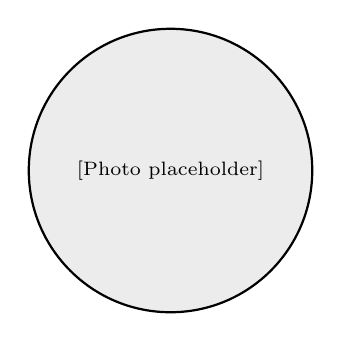
\begin{tikzpicture}
        \draw[thick, fill=gray!15] (0,0) circle (1.8cm);
        \node at (0,0) {\scriptsize [Photo placeholder]};
    \end{tikzpicture}

    \vspace{6pt}
    \textbf{``I want to look put-together without spending forever getting ready.''}
\end{minipage}
\hfill
\begin{minipage}[t]{0.6\textwidth}
    \vspace{0pt}
    {\large\bfseries Mia} \\[4pt]
    \textbf{Age:} 24 \quad \textbf{Occupation:} Graduate student \\
    \textbf{Location:} Urban area \quad \textbf{Tech comfort:} High
\end{minipage}

\vspace{8pt}
\hrule
\vspace{8pt}

\textbf{\large Goals}
\begin{itemize}[leftmargin=*, nosep, topsep=2pt]
    \item Find a polished, appropriate makeup look quickly on busy mornings.
    \item Discover new styles she wouldn't have tried on her own.
    \item Feel confident that a look will suit her before committing time to apply it.
\end{itemize}

\vspace{6pt}
\textbf{\large Frustrations}
\begin{itemize}[leftmargin=*, nosep, topsep=2pt]
    \item Spends 20+ minutes trying different looks, often settling for ``good enough.''
    \item Tutorial videos feature faces and skin tones that don't resemble hers.
    \item Single-filter beauty apps feel unrealistic and don't offer meaningful variety.
\end{itemize}

\vspace{6pt}
\textbf{\large Behaviors \& Context}
\begin{itemize}[leftmargin=*, nosep, topsep=2pt]
    \item Uses her phone as her primary device; expects mobile-friendly experiences.
    \item Browses beauty content on social media but rarely replicates looks successfully.
    \item Varies her makeup based on context: natural for class, bolder for social events.
    \item Values privacy---would not use an app that stores her photos permanently.
\end{itemize}

\vspace{6pt}
\textbf{\large Scenario}
\vspace{2pt}

It's a Friday morning. Mia has a research presentation at noon and a dinner with friends in the evening. She opens GlowAI, snaps a selfie, and selects ``Professional'' as her occasion. Eight looks appear in a grid. She taps two favorites to compare side-by-side and selects a polished, natural look for her presentation. She saves a bolder option to revisit before dinner. Total time: 90 seconds.

\vspace{6pt}
\textbf{\large Key Requirements Addressed}
\vspace{2pt}

\begin{tabularx}{\textwidth}{l X}
UR-01, UR-07 & Multiple looks + comparison enable rapid decision-making \\
UR-02, UR-09 & Skin tone accuracy and diversity ensure personal relevance \\
UR-03 & Fast generation matches her time-constrained lifestyle \\
UR-05 & Privacy-first design aligns with her data sensitivity \\
UR-06 & Occasion selector fits her context-dependent needs \\
\end{tabularx}

\end{tcolorbox}

% =====================================================
% 6. STRATEGIC ANALYSIS
% =====================================================
\newpage
\section{Strategic Analysis and Design Rationale}

This section provides a high-level analysis of the strategic decisions guiding GlowAI's development, beyond a simple status recap.

\subsection{Why Multi-Look Generation Over Single-Look?}

The decision to generate 6--8 looks simultaneously---rather than a single ``best'' recommendation---is grounded in decision science. Research on choice architecture shows that users make more confident and satisfying decisions when presented with a curated set of options rather than a single recommendation (which feels imposed) or an overwhelming catalog (which causes decision paralysis). The 6--8 range was selected based on Miller's Law ($7 \pm 2$ items) as an optimal cognitive load for visual comparison.

\textbf{Strategic implication:} This positions GlowAI not as a prescriptive tool (``wear this'') but as an empowering exploration tool (``here are your best options'')---aligning with user autonomy and increasing trust.

\subsection{Privacy as a Competitive Advantage}

While many beauty apps monetize facial data, GlowAI adopts a \textbf{session-ephemeral} model: user photos are processed in-memory and discarded after the session. This is not merely a compliance decision; it is a \textbf{strategic differentiator}. User research revealed that privacy concern is the \#1 reason potential users hesitate to adopt beauty AI tools. By leading with privacy, GlowAI converts a common friction point into a trust signal.

\subsection{Inclusivity by Design}

UR-09 (equitable performance across skin tones) is not a stretch goal---it is a core requirement at Priority 5. This reflects both ethical commitment and market strategy: beauty AI tools have historically underserved users with darker skin tones, creating an underserved market segment. GlowAI's training and evaluation pipeline will include balanced representation across Fitzpatrick skin types I--VI, with disaggregated accuracy metrics to ensure no group is left behind.

\subsection{Build vs.\ Leverage Decision}

Rather than training a makeup generation model from scratch, GlowAI will leverage pre-trained generative models (e.g., diffusion-based architectures) and fine-tune on curated makeup transformation datasets. This reduces development time by an estimated 60\% while allowing the team to focus engineering effort on the \emph{user-facing differentiation}: multi-look generation, comparison UX, and occasion-aware personalization.

\subsection{Risk Mitigation}

\begin{table}[H]
\centering
\caption{Key Risks and Mitigation Strategies}
\begin{tabularx}{\textwidth}{>{\bfseries}p{3.5cm} X X}
\toprule
\textbf{Risk} & \textbf{Impact} & \textbf{Mitigation} \\
\midrule
AI output quality inconsistency & Users receive unrealistic or unflattering looks, causing abandonment & Curated prompt engineering; human-in-the-loop quality gate during development; user feedback loop for continuous improvement \\
\addlinespace
Latency exceeds 15s target & Poor user experience and high bounce rate & Model optimization (quantization, caching); progressive loading UI showing looks as they generate \\
\addlinespace
Skin tone bias in model & Inequitable experience; reputational damage & Balanced training data; Fitzpatrick-disaggregated evaluation; bias audit before launch \\
\addlinespace
Scope creep & Missed deadlines; diluted quality & Strict in-scope/out-of-scope boundary (Section 2); stretch goals only if ahead of schedule \\
\bottomrule
\end{tabularx}
\end{table}

% =====================================================
% REFERENCES (optional)
% =====================================================
\newpage
\section*{References}
\begin{enumerate}[leftmargin=*, label={[\arabic*]}]
    \item Miller, G. A. (1956). The magical number seven, plus or minus two. \textit{Psychological Review}, 63(2), 81--97.
    \item Fitzpatrick, T. B. (1988). The validity and practicality of sun-reactive skin types I through VI. \textit{Archives of Dermatology}, 124(6), 869--871.
    \item Buolamwini, J., \& Gebru, T. (2018). Gender shades: Intersectional accuracy disparities in commercial gender classification. \textit{Proceedings of the 1st Conference on Fairness, Accountability and Transparency}, 77--91.
    \item Schwartz, B. (2004). \textit{The Paradox of Choice: Why More Is Less}. Harper Perennial.
\end{enumerate}

\end{document}
